\section{Solution} \label{sec:solution}
The solution we propose to the problem statement, introduced in the introduction, is as follows:
\begin{itemize}
	\item	Input a configuration that specifies all of the payloads, environment, and validation options
	\item	Produce a \gls{cora} model that will find the a optimal schedule
	\item	Validate the schedule in \gls{smc} to test the robustness and act accordingly to the result
	\begin{itemize}
		\item	Rejected: modify the configuration and produce a new schedule for validation
		\item	Accepted: output schedule along with robustness results
	\end{itemize}
\end{itemize}

By doing so we are able to produce a optimal schedule that is verified in regards to the robustness.
It is optimal in regards to profit while upholding certain restrictions, such as minimum acceptable battery level.
How the schedule is generated and how the robustness is tested will be explained in the following chapters of this report.
Prior to defining how the configuration is set in \cref{sec:read_input} \nameref{sec:read_input}, we will present our tool-chain which provides an overview of how the final system will work and how the different tools are used.

\subsection{Tool-chain} \label{subsec:tool_chainv}
In order to clarify our usage of different tools we will describe the different steps in our system. 
\Cref{fig:tool1} displays a flowchart representation of the tool-chain.

\begin{figure}[h]
	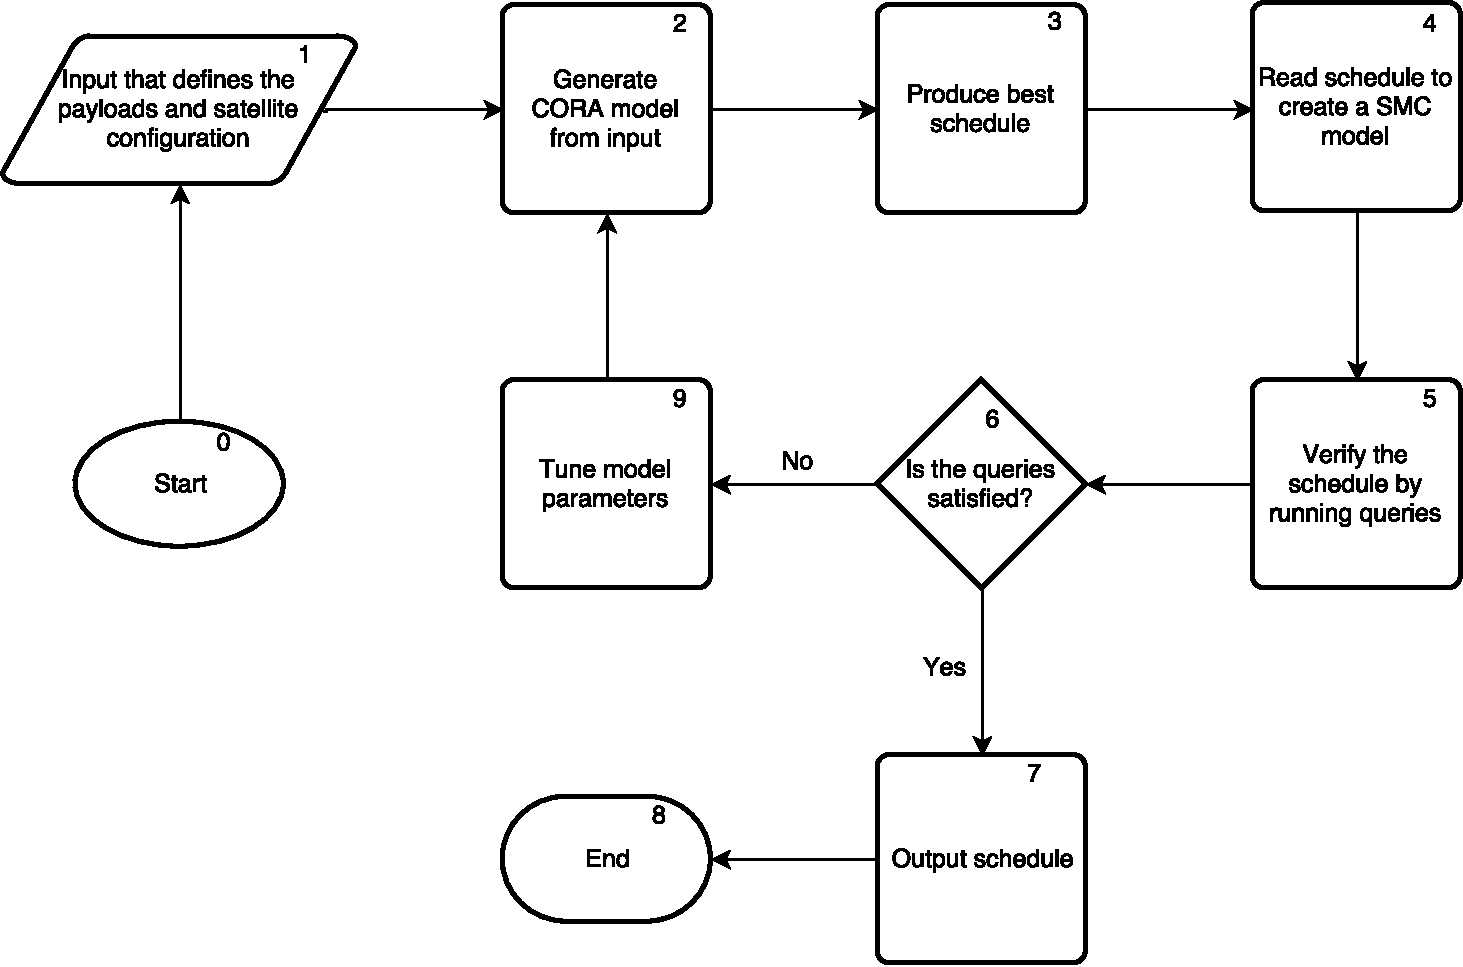
\includegraphics[width=\textwidth]{graphics/flow_final.pdf}
	\caption{Flowchart that displays the workflow and use of tools}
	\label{fig:tool1}
\end{figure}

\paragraph{Location 1 - Input that defines the payloads and nanosatellite configuration} 
The configuration for the system is read in order to properly model the nanosatellite and its payloads.

\paragraph{Location 2 - Generate \gls{cora} models from input} 
The payloads, windows, and other variables is modelled in the UPPAAL \gls{cora} model, as specified by the input configuration.

\paragraph{Location 3 - Produce best schedule} 
Make UPPAAL \gls{cora}  produce the schedule.

\paragraph{Location 4 - Read schedule to generate a UPPAAL \gls{smc} model}
The model is able to simulate the execution of the schedule and test for robustness.

\paragraph{Location 5 - Verify the schedule by running queries} 
UPPAAL \gls{smc} will run the queries on the model and output the results, see \cref{sec:smc}. 
These queries is made to validate and test the robustness of the schedule.

\paragraph{Location 7 - Output schedule} 
If the queries are satisfied we will output the schedule, as this will indicate that the trace, or schedule, is correct.

\paragraph{Location 9 - Tune model parameters} 
If the queries were not satisfied, the schedule will be discarded and we will produce a new one. 
In order to produce a new schedule, we will provide UPPAAL \gls{cora} with a new configuration. 
The configuration will be loyal to the one specified by the user, but certain values will be changed, such as the time to complete a payload, in order to provoke new choices in the schedule. 
